\documentclass{article}

\usepackage[english]{babel}
\usepackage[utf8]{inputenc}
\usepackage[]{hyperref}
\usepackage{graphicx, float}
\usepackage{subfig}
\usepackage{amssymb, amsmath, amsthm, stmaryrd}

%%%%%%%%%%%%%%%% Lengths %%%%%%%%%%%%%%%%
\setlength{\textwidth}{15.5cm}
\setlength{\evensidemargin}{0.5cm}
\setlength{\oddsidemargin}{0.5cm}

%%%%%%%%%%%%%%%% Variables %%%%%%%%%%%%%%%%
\def\projet{6}
\def\titre{Résolution approchée d'équations différentielles ordinaires}
\def\groupe{4}
\def\equipe{4}
\def\responsible{}
\def\secretary{}
\def\others{}

\begin{document}

%%%%%%%%%%%%%%%% Header %%%%%%%%%%%%%%%%
\noindent\begin{minipage}{0.98\textwidth}
	\vskip 0mm
	\noindent
	{ \begin{tabular}{p{7.5cm}}
		{\bfseries \sffamily
			Projet \projet} \\ 
		{\itshape \titre}
		\end{tabular}}
	\hfill 
	\fbox{\begin{tabular}{l}
		{~\hfill \bfseries \sffamily Group \groupe\ - Team \equipe
			\hfill~} \\[2mm] 
		Manager : \responsible \\
		Secretary : \secretary \\
		Programmer : \others
		\end{tabular}}
	\vskip 4mm ~

	~~~\parbox{0.95\textwidth}{\small \textit{Summary~:} \sffamily
		Résumé à faire ici.
	}
	\vskip 1mm ~
\end{minipage}

%%%%%%%%%%%%%%%% Main part %%%%%%%%%%%%%%%%

\section{Résolution d'équations différentielles ordinaires}\label{sec:sec1}
Les algorithmes de résolution présentés ici utilisent tous des méthodes avec un pas de discrétisation, de la forme
$y_{n+1}=y_n+h_n \times \phi (y_n,t_n,h_n)$. En pratique, on cherche à mettre l'équation différentielle sous la forme d'un produit de Cauchy.
Cela fait intervenir une fonction $f$ et une fonction $y$ ainsi que sa dérivée, ainsi qu'un vecteur de conditions initiales $y_0$.
On a alors $y'(t)=f(y(t),t)$, et $y(t_0)=y_0$.

\subsection{Méthodes de résolution}
Nous avons implémenté les méthodes de résolution d’Euler, du point-milieu, de Heun et de Runge-Kutta.
Ces méthodes se basent sur des équations donnant $y_{n+1}$ en fonction de $y_n$, $h_n$ et $t_n$.

Une fonction a donc été réalisée pour chacune de ces méthodes, et permet d'effectuer un unique pas de temps.
Les fonctions détaillées dans la suite réutiliseront ces fonctions, en effectuant un nombre d'itérations défini, selon la méthode choisie.

Nous avons implémenté \texttt{meth\_n\_step} qui calcule un nombre $N$ d'étapes avec un pas constant $h$,
puis \texttt{meth\_epsilon} qui calcule une solution approchée avec un paramètre d’erreur $\epsilon$.
Une fois adaptée, cette dernière fonction permet de visualiser la convergence de la solution en fonction du nombre de subdivisions,
comme le montre la figure~\ref{fig:subdivision}.
En pratique, à chaque itération, si l'erreur entre deux itérations successives est inférieure à $\epsilon$,
alors on arrête le calcul et on renvoie la solution.

\begin{figure}[htbp!]
	\centering
	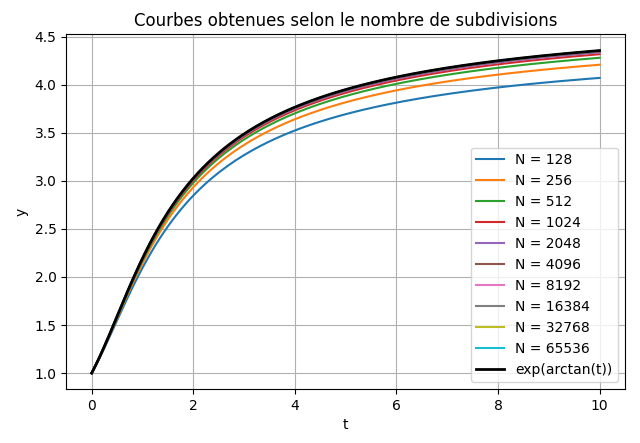
\includegraphics[width=0.45\textwidth]{res/subdivisions}
	\caption{Solutions obtenues en fonction du nombre de subdivisions, pour $y'(t) = \frac{1}{1 + t^2}$ avec $y(0) = 1$.}
	\label{fig:subdivision}
\end{figure}

Comme attendu, on observe une convergence de la solution vers la solution exacte (tracée en noir)
lorsque le nombre de subdivisions augmente.

Sur l'ensemble des méthodes de résolution étudiées, la plus précise est celle de Runge-Kutta, puisqu'elle est d'ordre $4$.
En revanche, c'est aussi la plus coûteuse en temps, puisqu'elle nécessite quatre appels à la fonction $f$ pour un unique pas de temps.
La méthode d'Euler est la moins précise (ordre $1$), mais la plus rapide, puisqu'elle ne nécessite qu'un seul appel à la fonction $f$ par pas de temps.
Les autres méthodes constituent un bon compromis entre précision et temps de calcul, puisque celle du point-milieu et de Heun sont d'ordre $2$, et nécessitent deux appels à la fonction $f$.

\subsection{Champ des tangentes}
Pour continuer, nous avons implémenté la fonction \texttt{tangent\_2D} permettant de tracer le champ des tangentes,
pour les équations différentielles de dimension $2$.

La figure~\ref{fig:tangente}, montre le champ des tangentes sur une équation différentielle
de dimension $2$, à savoir $y(t)=(y_1(t),y_2(t))$, avec $y(0)=(1,0)$ et $y'(t)=(-y_2(t),y_1(t))$.
Les résultats obtenus semblent cohérents par rapport aux résultats réels.

\begin{figure}[htbp!]
	\centering
	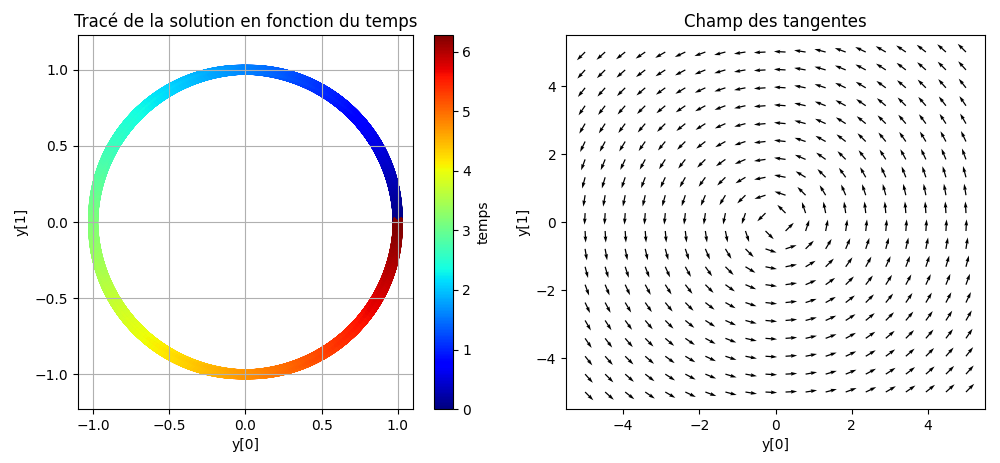
\includegraphics[width=0.7\textwidth]{res/tangente}
	\caption{Solution de l'équation différentielle, et son champ des tangentes}
	\label{fig:tangente}
\end{figure}

\vspace*{-0.7cm}
\label{sec1}

\section{Système proie-prédateur de Lotka-Volterra}\label{sec:sec2}
Dans cette partie, nous allons étudier le système proie-prédateur de Lotka-Volterra,
qui est un système d'équations différentielles ordinaires,
et le comparer à des modèles plus simples.


\subsection{Modèles simplistes}
Un des premiers modèle de population est celui de Malthus, qui suppose une croissance exponentielle de la population $N(t)$.
Celui-ci utilise l'équation $\frac{dN(t)}{dt} = \gamma N(t)$, avec $\gamma \in \mathbb{R}$.

Un coefficient $\gamma$ positif implique une croissance de la population, et un coefficient négatif une décroissance.
Un autre modèle a été proposé, celui de Verhulst, utilisant une formule similaire à celle de Malthus,
à la différence qu'il ne croît pas au delà d'une certaine population $\kappa$, ce qui simule une limite de ressources.
Il utilise l'équation $\frac{dN(t)}{dt} = \gamma N(t) \left( 1 - \frac{N(t)}{\kappa} \right)$,
avec $N(t)$ la population à l'instant $t$ (à un facteur près), $\gamma \in \mathbb{R}$ et $\kappa \in \mathbb{R}$.

Les résultats de ces deux modèles sont présentés sur la figure~\ref{fig:populations}, ce qui montre bien que le modèle de Verhulst
est plus réaliste que celui de Malthus.

\begin{figure}[htbp!]
	\centering
	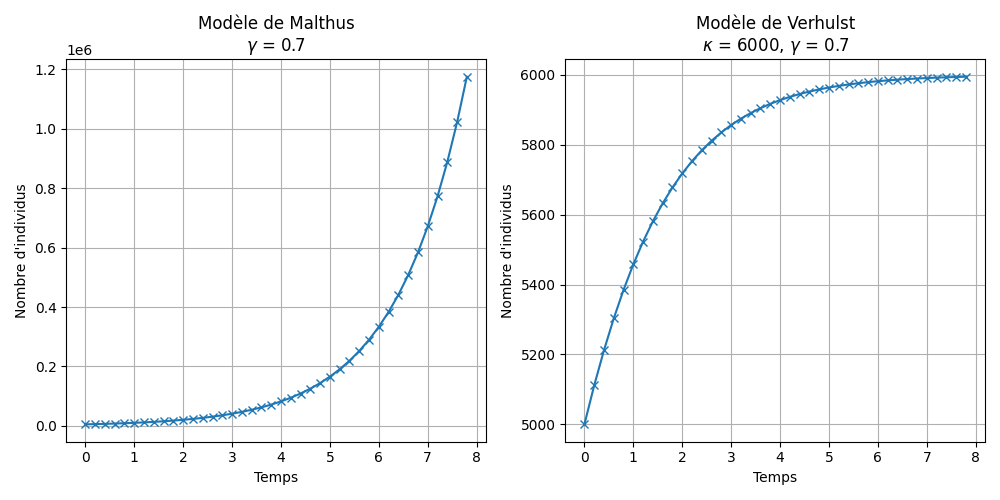
\includegraphics[width=0.7\textwidth]{res/population}
	\caption{Comparaison des modèles de Malthus et de Verhulst, avec initialement $40$ individus.}
	\label{fig:populations}
\end{figure}

Le modèle de Lotka-Volterra est un modèle plus réaliste, qui prend en compte deux populations,
l'une de proies, l'autre de prédateurs.
Il utilise les équations~\ref{eq:lotka}, avec $N(t)$ la population de proies à l'instant $t$ (à un facteur près),
$P(t)$ la population de prédateurs à l'instant $t$, $(a, b, c, d) \in (\mathbb{R}^{+*})^4$.

\begin{equation}
	\label{eq:lotka}
	\frac{dN(t)}{dt} = N(t) \times (a - b \times P(t)) \ \ \ \ \ \ \ \ \ \ \ \ \ \ \
	\frac{dP(t)}{dt} = P(t) \times (c \times N(t) - d)
\end{equation}

Après résolution avec \texttt{meth\_epsilon}, on obtient la figure~\ref{fig:lotka}, qui montre une solution périodique.

\begin{figure}[htbp!]
	\centering
	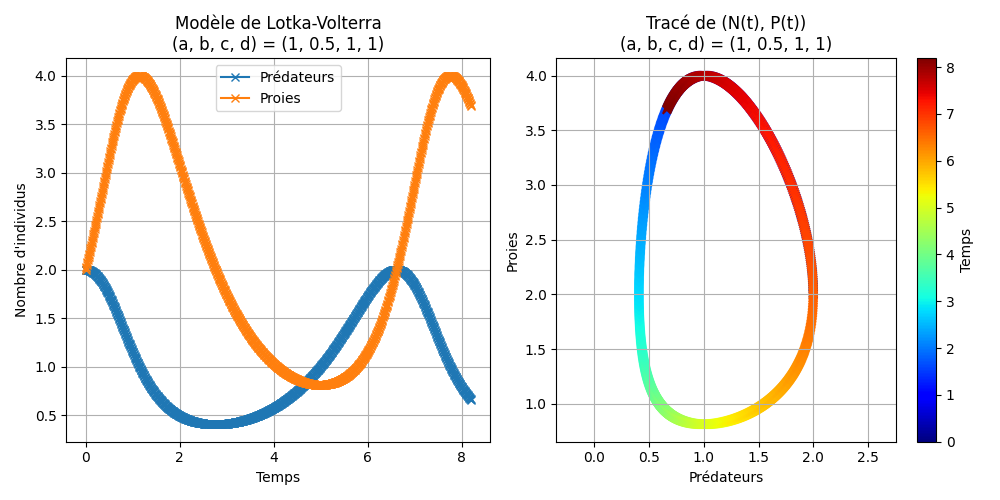
\includegraphics[width=0.7\textwidth]{res/lotka}
	\caption{Résolution du système de Lotka-Volterra, avec initialement $2$ proies et $2$ prédateurs.}
	\label{fig:lotka}
\end{figure}

De sorte à calculer rapidement la période des oscillations des deux populations, on itère
sur les valeurs échantillonnées, et on vérifie si la valeur actuelle est proche de la toute première.

Concernant les solutions constantes pour ce modèle, elles sont obtenues pour des dérivées nulles,
ce qui se traduit par la formule logique~\ref{eq:lotka-const}. Ce sont les points singuliers
de l'équation différentielle.

\begin{equation}
	\label{eq:lotka-const}
	\left(\left(N(t) = 0\right) \vee \left(P(t) = \frac{a}{b}\right)\right)
	\wedge
	\left(\left(P(t) = 0\right) \vee \left(N(t) = \frac{d}{c}\right)\right), \forall t \in \mathbb{R}
\end{equation}

En traçant les solutions proches d'un point non-singulier, on obtient la figure~\ref{fig:behaviour}. Systématiquement,
pour des points non-singuliers, on obtient des solutions périodiques, et donc un cycle fermé, de forme déterminée par les paramètres.
Pour des points singuliers, on a des ellipses si les valeurs ne sont pas nulles, selon la formule~\ref{eq:lotka-const},
et des droites si l'une des valeurs est nulle, sinon un point.

\begin{figure}[htbp!]
	\centering
	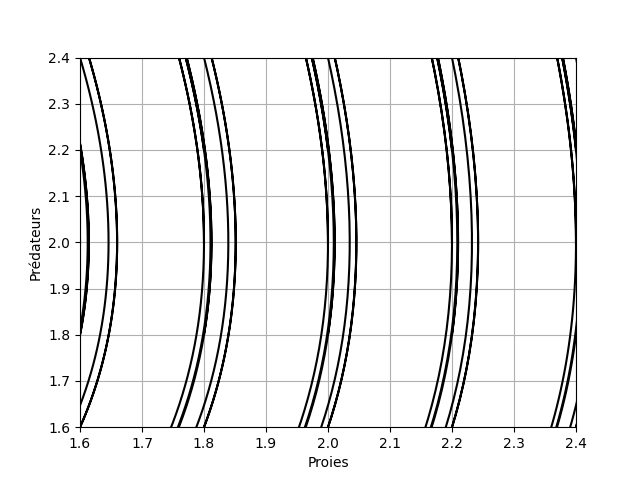
\includegraphics[width=0.45\textwidth]{res/behaviour}
	\caption{Comportement des solutions proches d'un point non-singulier (rectangle autour de $(2, 2)$)}
	\label{fig:behaviour}
\end{figure}

Dans le cas général, pour une équation différentielle quelconque, il n'y a pas nécessairement de cycle fermé dans une représentation
telle que celle de la figure~\ref{fig:behaviour}.
\label{sec2}

\section{Pendule à $N$ maillons}

\renewcommand*{\overrightarrow}[1]{\vbox{\halign{##\cr 
  \tiny\rightarrowfill\cr\noalign{\nointerlineskip\vskip1pt} 
  $#1\mskip2mu$\cr}}}

Dans cette partie, nous allons considérer deux types de pendules à $N$ maillons (le pendule simple et le pendule double) et chercher à 
résoudre leurs équations de mouvement par les méthodes numériques implémentées dans la section~\ref{sec:sec1}.

\subsection{Pendule simple}
Dans le cas du pendule simple, il y a deux forces qui s'appliquent sur la masse $m$:
le poids de la masse \overrightarrow{P} et la force de la tige \overrightarrow{T}.
Selon le théorème du moment cinétique appliqué en $M$ par rapport à $O$, on a
$\frac{d\overrightarrow{L_{O,M}}}{dt} = \overrightarrow{M_{O, M}(\overrightarrow{P})} + \overrightarrow{M_{O, M}(\overrightarrow{T})}$.

Le moment de \overrightarrow{T} est nul, car \overrightarrow{OM} et \overrightarrow{T} sont colinéaires. En développant l'expression, on a alors 
$m l^{2} \ddot \theta = - m l g \sin{\theta} $, ce qui nous donne finalement l'équation $\ddot \theta + \frac{g}{l} \sin{\theta}= 0$.

On retrouve l'équation différentielle non linéaire du second ordre bien connue du pendule simple. 
Pour la résoudre numériquement en fonction de l'angle initial $ \theta_0 $, et de la vitesse initiale $ \dot \theta_0 $,
on peut utiliser une des méthodes implémentées auparavant, comme par exemple la méthode d'Euler.
Une fois que la fonction $ \theta(t) $ a été approchée, on peut calculer la période du pendule en prenant la différence entre 
deux maxima successifs, ce qui permet de déterminer la fréquence.

En affichant les différentes fréquences du pendule pour des valeurs de $ \theta_{0} $ variant de $ -\frac{\pi}{2} $ à $ \frac{\pi}{2} $, 
on obtient la figure~\ref{fig:frequences}.

\begin{figure}[htbp!]
	\centering
	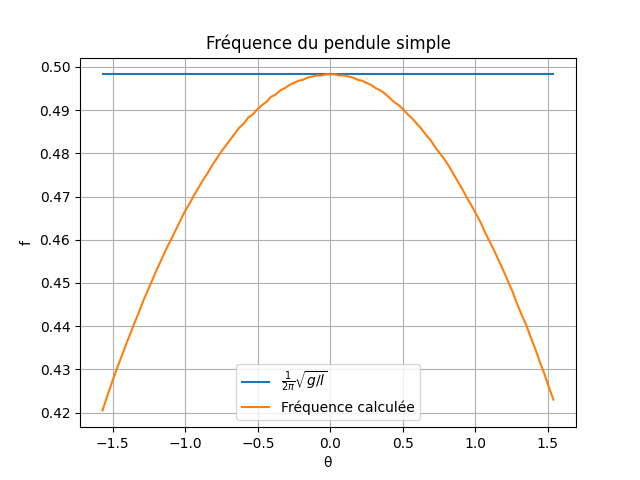
\includegraphics[width=0.45\textwidth]{res/freq_pendule_simple.png}
	\caption{Fréquence du pendule en fonction de l'angle initial $ \theta_{0}$}
	\label{fig:frequences}
\end{figure}

On remarque bien que pour des valeurs de $ \theta_0 $ faibles représentant les petites oscillations du pendule, 
la fréquence semble bien égale à la valeur $ \frac{1}{2 \pi} \sqrt{\frac{g}{l}} $.

\subsection{Double pendule}
Le pendule à deux maillons est constitué de deux masses $ m_1 $ et $ m_2 $ 
reliées par deux tiges de longueur $ l_1 $ et $ l _2 $. On note $ \theta_1 $ et $ \theta_2 $ les angles
que font les tiges avec la verticale. Dans la littérature, on trouve les deux équations donnant $\ddot \theta_1$ et $\ddot \theta_2$ en fonction des autres paramètres.

La mise sous forme du système d'équations différentielles comme précisé en première partie est plus complexe,
puisqu'il faut passer par un vecteur de résolution de dimension $4$.
En effet, le système possède $4$ conditions initiales, à savoir les angles initiaux, et les vitesses initiales.
On a donc le vecteur $ U = (\theta_1, \theta_2, \dot \theta_1, \dot \theta_2) $, et on peut donc écrire sa dérivée en fonction de ses variables, et des équations donnant $\ddot \theta_1$ et $\ddot \theta_2$,
ce qui nous donne le vecteur $ U' = (\dot \theta_1, \dot \theta_2, \ddot \theta_1, \ddot \theta_2) $.

\medbreak

Les croix représentent le début du parcours de l'extrémité de chaque pendule.
On remarque que les trajectoires suivent tout d'abord le même chemin puis divergent complètement au cours du temps.

À l'inverse du pendule simple où les trajectoires sont des ellipses peu importe les conditions initiales, 
le pendule double est quant à lui un système très sensible à celles-ci: c'est un système chaotique.  

\medbreak

Une fois les trajectoires calculées, on peut s'intéresser au temps que met le pendule à se retourner (la masse $ m_2 $ passe au
dessus de $ m_1 $).
Ce retournement arrive lorsque $ \theta_2 $ dépasse en valeur absolue $ \pi $.
Pour des valeurs faibles des conditions initiales, on peut observer que le pendule ne se retourne pas, comme dans la figure~\ref{fig:no_retournement}.
En revanche, lorsqu'on augmente les vitesse angulaires, on peut généralement observer un retournement du pendule, comme dans la figure~\ref{fig:retournement}.
Ces deux figures ont été tracées avec des conditions initiales nulles, excepté pour la vitesse angulaire $ \dot \theta_2 $.

\begin{figure} [htbp!]
	\begin{minipage}[c]{0.45\textwidth}
		\centering
		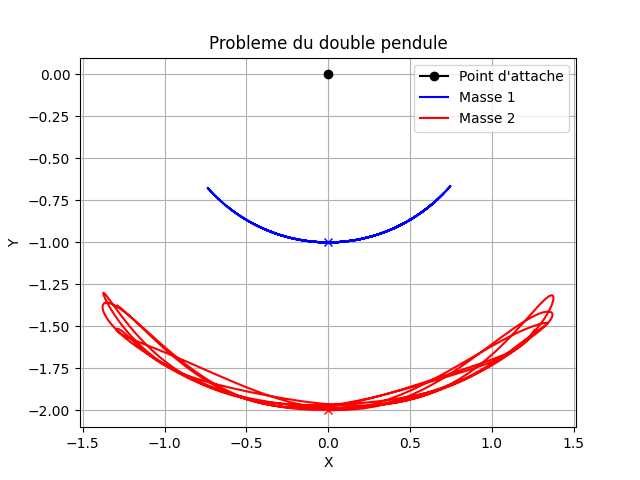
\includegraphics[width=\textwidth]{res/no_retournement.png}
		\caption{Pas de retournement, $\dot \theta_2 = 4$ rad}
		\label{fig:no_retournement}
	\end{minipage}\hfill
	\begin{minipage}[c]{0.45\textwidth}
		\centering
		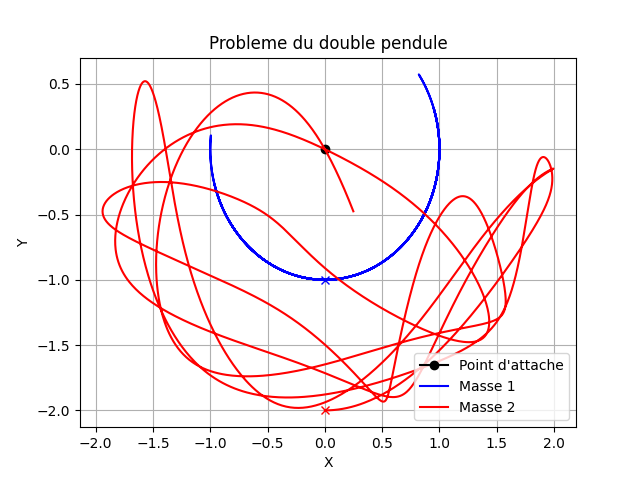
\includegraphics[width=\textwidth]{res/retournement.png}
		\caption{Retournement, $\dot \theta_2 = 8$ rad}
		\label{fig:retournement}
	\end{minipage}
\end{figure}
\label{sec3}

\end{document}